\chapter{Korrespondance Analyse} \label{sec:Kor}
Korrespondance problemet, imellem to eller flere billeder af samme objekt, referere til problemet om at finde et sæt af punkter i det ene billede, der kan identificeres og matches i det andet.
Udfordringen ved problemet ligger i at billederne, der skal matches, er udsat for en række ændringer, det kan f.eks. være forskydning i kameraets position ift. scenen eller  ændringer i scenens motiv. Et godt eksempel på korrespondance problemet er det menneskelige syn. Øjnene agere som to kameraer, der hver især fanger deres billede og omdanner disse billeder til et sammenhængende panoramisk billede, ved hjælp af oprettelse af korrespondancer. Korrespondancen mellem øjnene tillader også opfattelse dybde i billedet, hvilket skyldes den horisontale forskydning af menneskets øjne. Denne sektion vil beskrive, hvordan denne korrespondance kan efterlignes af en computer
\begin{figure}[H]
    \centering
    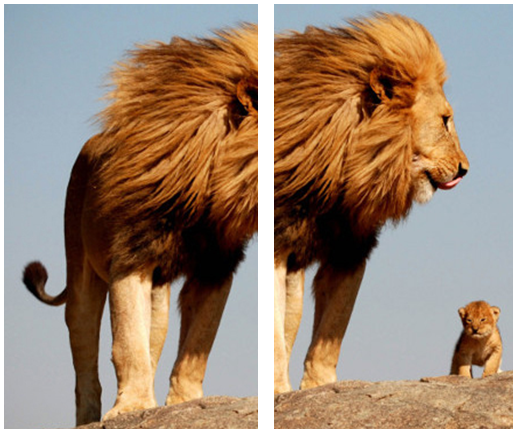
\includegraphics[width=0.45\textwidth]{fig/3.png}
     \vspace{-1em}
    \begin{center}    
       \caption{\textcolor{gray}{\footnotesize \textit{To billeder er af samme 2-D motiv, med kamerapositionen forskudt i x-aksen.}}}
    \label{fig:1}
     \end{center}
     \vspace{-2.5em}
  \end{figure} \noindent
I figur \ref{fig:1} ses to billeder af det samme motiv, men hvor kameravinklen er forskudt. For at opnå en korrespondance imellem billederne skal der detekteres nogle unikke punkter, som skal optræde i begge billeder, dvs. der hvor billederne overlapper. Punkterne skal nøje beskrives så de kan genkendes i transformerede billeder. Til sidst skal punkterne matches for at estimere hvordan de korrespondere med hinanden, altså i dette tilfælde, hvordan de er forskudt i forhold til hinanden. Korrespondance analysens pipeline, der består af feature detektion, deskription og matching, er yderligere beskrevet herunder.
\section{Detektor}
Feature detektion er en metode indenfor billedbehandling, der determinere, for hvert punkt i et billede, om dette punkt er et interessepunkt. Interessepunktet er ofte fundet ved at evaluere et pixel område omkring det fundne punkt. Detektorens resultat vil derved være et subset af isolerede punkter fra billedet, der er markeret som interessante. (Så hvornår er punkter interessante?) Om et punkt er interessant, defineres udefra hvilke egenskaber der er interessante for applikationsdomænet. Det kan f.eks. være genkendelse af veje fra satellitbilleder, ved at finde kanter eller linjer.  Interesse punkter defineres ikke udefra semantiske meningsfulde områder som ansigter eller objekter, da dette vil kræve en høj-niveau fortolkning af scenen. I stedet udvælges lokale pixel områder, der er matematisk distinktive, baseret på intensiteten i billedet. Der er mange måder at definere hvad et interessepunkt er og det er i sidste ende applikationsdomænet der afgør hvilke punkter der lokaliseres bedst, det kan dog overordnet defineres at en detektor skal besidde følgende egenskaber:
\begin{itemize}
\item{\emph{Repeterbar}: Givet to billeder, taget af samme objekt under forskellige betingelser, skal en stor  del af de fundne punkter uafhængigt af hinanden, indgå i begge billeder. Lokaliseres punkterne ikke tilstrækkeligt i begge billeder er det ikke muligt at oprette en korrespondance
}
\item{ \emph{Distinkte:}
 De fundne interessepunker skal være unikke ift. intensitetsvariationen i det omkringliggende område. Dette muliggør bedere beskrivelse af punktet og derved større mulighed for korrekt match.}
\end{itemize}
Disse egenskaber kan opnås ved følgende:
\begin{itemize}
\item{ \emph{Invarians:} Detektionsmetoden skal tage højde for de ændringer der kan forekomme i mellem billederne, og derved være invariante overfor disse. Det kan f.eks være rotation af kameraet under billedetagning osv.}
\item{ \emph{Robusthed} Detektoren skal være robust overfor små deformationer som støj i billedet, hvilket fejlagtigt kan fortolkes som interessepunkter.}
\end{itemize}
Udvælges punkterne ikke konsistent i begge billeder, er korrespondance oprettelsen ikke mulig. Nedenstående er en gennemgang af forskellige lokale mønstre som kan bruges til udvælgelse af interessepunkter.
 \subsection{Hjørner}
En hjørnedetektor, leder efter hjørner i billedet og anvender disse som interessepunkter. Et hjørne kan defineres ved et punkt der har to dominerende kanter i hver sin retning.
\begin{figure}[H]
    \centering
    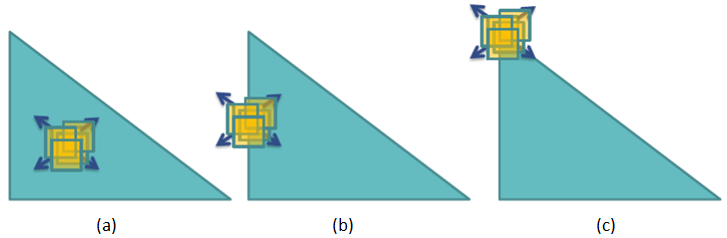
\includegraphics[width=0.55\textwidth]{fig/6.png}
    \vspace{-1em}   
    \begin{center}    
    \caption{\textcolor{gray}{\footnotesize \textit{
     Tre udvalgte vinduer, med interessepunkter i centrum af samme motiv. \textbf{(a)} Punktet er lokaliseret i en teksturløs region, d.v.s. ingen teksturskift. \textbf{(b)} Punktet er lokaliseret på en kant. \textbf{(c)} Punktet er lokaliseret på et hjørne }}}
    \label{fig:2}
     \end{center}
    \vspace{-2.7em}  
  \end{figure}  
\noindent
Hvorfor er hjørner gode punkter? Et hjørne er et godt interessepunkt da der foregår store intensitetsskift omkring hjørnets omliggende område og er derfor distinkt ift. området.
En intuitiv måde at definere hvorfor et punkt er interessant, er at placere et firkantet vindue omkring punktet. Dette vindue forskydes lokalt i x og y retningen. Resultere forskydningen af interessepunktet i  et nyt objekt identisk med interessepunktet er punktet ikke lokalt distinkt. På figur \ref{fig:2} ses tre udvalgte punkter med et firkantet vindue placeret over. I stil med ovenstående definition, forskydes det firkantede vindue i alle retninger. Forskydes \textbf{(a)} vil det matche alle de forskudte billeder da regionen omkring punktet også er teksturløst. Punktet er derfor ikke distinkt. Forskydes \textbf{(b)} i x-aksen opnås et nyt objekt, men en forskydning i y-aksen vil resultere i samme objekt, og \textbf{(b)} er derfor ikke distinkt. Punktet placeret på et hjørne er distinkt da ingen forskydninger vil matche original billedet. Hjørnet kan derfor bruges som et distinktivt interessepunkt. At detektere hjørner er en udbredt teknik, da de er lokalt definerbare og ofte forekommer i forskellige scener. En matematisk definition kan opstilles og hele billedet og gennemsøges ift. definitionen.
\subsection{Kanter}
< intro gradient http://www.slideshare.net/grim42/fuzzy-logic-based-edge-detection >
\noindent
Kant detektion, referere til at finde kanter i billedet, hvor en kant kan defineres som et skarpt skift i billedintensiteten. Som nævnt er kanter ikke lokalt distinkte, men kan bruges til at fjerne en del unødvendig information fra et billedet, ved kun at udtrykke kanterne. 
En måde at visualisere definitionen af en kant, er ved at opfatte billedet som et signal, en intensitetsfunktion, der afbilder billedintensiteten i 1-dimension. En høj kurve, angiver et skarpt intensitetsskift og derved en kant. Kanter kan derved identificeres ved at finde disse skarpe sving i intensitetsfunktionen.
\noindent
\begin{figure}[H]
    \centering
    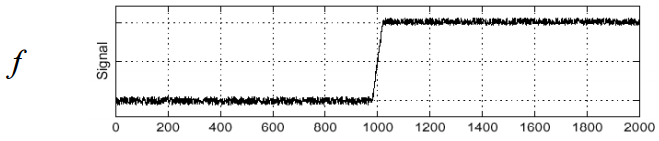
\includegraphics[width=0.55\textwidth]{fig/7.png}
     \vspace{-1em}
    \begin{center}        
     \caption{\textcolor{gray}{\footnotesize \textit{
     En 1-dimensional fortolkning af intensiteten i et billede. De små udsving indikere støj, den store kurve repræsenter et skrapt skift i intensiteten og derved en kant i et billedet.}}}
    \label{fig:kant}
     \end{center}
       \vspace{-2.5em}
  \end{figure}
\noindent
I figur \ref{fig:kant} er en kant visualiseret efter ovenstående definition. Kanten i figuren kan findes ved at differentiere funktionen.
En differentiering af funktionen vil angive, hvor skarp kurven er og derved fremhæve dens udsving. Et 2-dimensionelt billede er ikke en kontinuerlig funktion, og kan derved ikke differentieres i traditionel forstand, men består af diskrete værdier i form af pixel informationer.
Differentiering af en funktion \emph{f(x)} kan approksimeres til følgende diskret differentiering:
\begin{equation}
\dfrac{df(x)}{dx}=\dfrac{f(x+1)-f(x-1)}{2}
\label{diff}
\end{equation}
Ovenstående i \eqref{diff} kan opnås ved at folde billedet med kernen $[1,0,-1]$, hvor foldning af et billede \emph{I}, med en kerne \emph{K}: $I\oplus K$, hvor K har indgangen m x n og I M x N udregnes som:
\begin{equation}
O(i,j) = \sum\limits_{k=1}^m \sum\limits_{l=1}^m I(i+k-1,l-1)K(k,l)
\end{equation}
Hvor det nye punkt i billedet er $O(i,j)$. Ved differentiering fremhæves udsving i intensitetsskiftene i billederne, hvilket gør det muligt at identificere kanterne. Problemet ved dette, visualiseret i figur \ref{fig:kant}, er at støj i billedet (de små udsving) også vil blive fremhævet, hvilket vil resultere i fejlagtige detektioner af kanter. For at imødekomme dette foldes billedet med et gaussisk filter, hvilket er en approksimering til den gaussiske funktion. Den gaussiske funktion kan bruges, i billedbehandling, til at beskrive et punkt, ved en vægtet normalfordeling i de omliggende pixel, visualiseret som en klokke, der ligges over billedet. Foldningen med et gauss filter vil derfor resultere i en "flydende" overgang mellem pixels og derfor glatte billedet.  Den gaussiske funktion i 2-D, hvor $ \sigma $ er standart afvigelsen, der determinere graden af glatning, er defineret i \eqref{2dgaussian}.
\begin{equation}
G(x,y) = \frac{1}{2 \pi \sigma ^{2}} e^{- \frac{x^{2} + y^{2}}{2 \sigma ^{2}}}
\label{2dgaussian}
\end{equation}
Sigma værdien bestemmer, hvor meget et billede skal sløres. I figur \ref{fig:sigma} ses to billeder foldet med forskellige sigma værdier.
\begin{figure}[H]
    \centering
    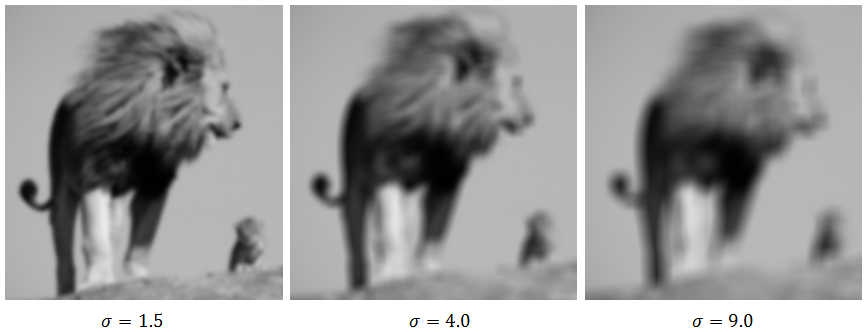
\includegraphics[width=0.65\textwidth]{fig/14.png}
    \vspace{-1em}
    \begin{center}    
    \caption{\textcolor{gray}{\footnotesize \textit{
     To billeder udsat for forskellige værdier i sigma.}}}     
    \label{fig:sigma}
    \vspace{-2.5em}
     \end{center}
\end{figure}
\noindent
For at undgå itereration af biledet to gange når kanter skal detekteres, for differentiering og sløring, kan dette udføres i en samlet operation ved at folde billedet med en differentieret gauss kerne, da foldning er en associativ operation,.
\begin{figure}[H]
    \centering
    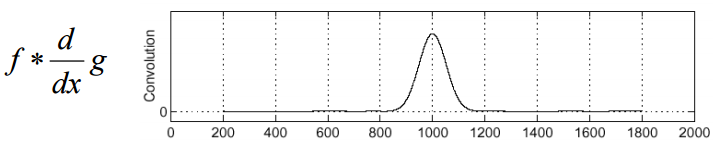
\includegraphics[width=0.55\textwidth]{fig/8.png}
    \vspace{-1em}   
    \begin{center}
    \caption{\textcolor{gray}{\footnotesize \textit{
     Resultatet af at folde et differentieret gauss filter på funktionen}}}
    \label{fig:deriv}
     \end{center}
    \vspace{-2.5em}  
  \end{figure}
\noindent
Kanterne er nu let definerbare som set i figur \ref{fig:deriv}. I et 2-dimensionelt billede repræsentere intensitetsskift også en orientering. Vertikale kanter findes ved at folde billedet med en gauss kerne differentieret i x-aksen og y-aksen for horisontale kanter som set i figur \ref{fig:deriv}.
\begin{figure}[H]
    \centering
    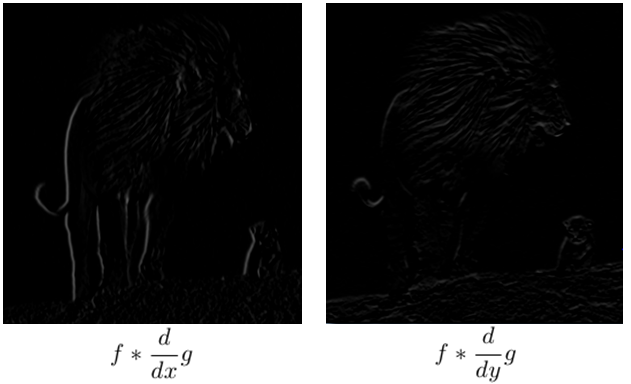
\includegraphics[width=0.45\textwidth]{fig/9.png}
    \vspace{-1em}   
    \begin{center}
    \caption{\textcolor{gray}{\footnotesize \textit{
     To billeder foldet med en differentieret gauss i x og y-aksen. Billedet viser tydeligt hvordan differentiering i x-aksen giver horisontale kanter og y-aksen giver vertikale kanter.}}}
    \label{fig:deriv}
     \end{center}
  \end{figure}
       \vspace{-2.5em} 
\noindent
\subsection{Blobs}
En blob detektor detektere regioner i billedet, hvor der sker en ændring af billedets egenskaber, det kan f.eks. være lysintensiteten ift. den omliggende region. En blob består af et sæt sammenhængnede pixels alle af samme intensitet, der er distinktive ift. området. Lindenberg \cite{blob} definere blobs som værende lyse regioner på sort baggrund eller omvendt, altså strukturere, der står i kontrast til deres baggrund. En blob kan derfor defineres som bestående af et område med \emph{mindst} ét lokalt ekstrema, enten et maksimum eller et minimum. Blobbens struktur er ikke semantisk intuitivt definerbar, men er matematisk veldefineret <?>.
\begin{figure}[H]
    \centering
    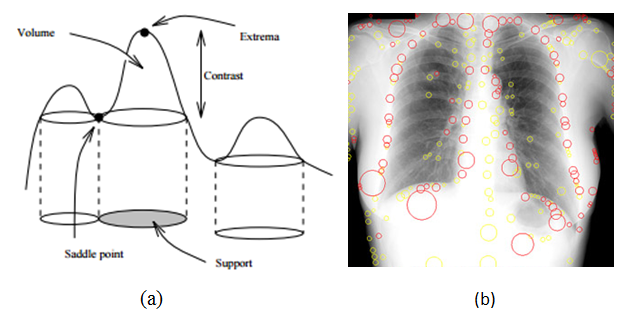
\includegraphics[width=0.65\textwidth]{fig/13.png}
    \vspace{-0.5em}   
    \begin{center}
    \caption{\textcolor{gray}{\footnotesize \textit{
    (a) En blob visualiseret i 2-d, udefra Lindenberg's definition. (b) En blob detektion udført på et røntgen billedet af en brystkasse, cirklerne angiver fundne blobs, og størrelserne på disse definere,  skalaen af disse blobs.}}}
    \label{fig:lindblob}
     \end{center}
  \end{figure}
       \vspace{-2.5em}
\noindent
I figur \ref{fig:lindblob}(a), ses en blob defineret af dets lokale ekstrema, hvor styrken af blobben beksrives ved kontrasten, ift. området omkring ekstrema. Lindenberg definere blobbens domæne som værende afgrænset af dens "saddle point". Et "saddle point" angiver punktet, hvor intensiteten stopper med at falde og starter med at stige for lyse blobs, og modsat for mørke. Punktet definere altså hvordan blobben er lokalt præsenteret. Denne definition på en blob stemmer overens med definitionen af interessepunkter. Det lokale ekstrema gør blobben vel defineret i regioner af billedet og derved distinktive. Blobs har også en fordel ift. kant og hjørne detektion, da blobs indgår i de fleste domæner undtagen homogene billeder. Kanter og hjørner forekommer ofte i menneskeskabte objekter, ved veldefinerede strukturer. Blobs har derfor flere applikationsområder, og kan bruges indenfor billeder af objekter, der ikke er menneskelige defineret scener, f.eks. indenfor medicinsk billedanalyse til detektion af anomalier i røngten billeder som set i figur \ref{fig:lindblob}(b). 
Ligesom i kant-detektion, kan blobs beskrives ved intensitetsskift, hvor der forekommer en krusning rundt om ekstremaet. En metode til at detektere disse ekstremaer hedder Laplacian operatoren $\Delta^2$. Laplace operatoren anvendes på et gaussisk filter og opnår operatoren "Laplacian of Gaussian" \eqref{lap}:
\begin{equation}
\Delta^2 f = \dfrac{\partial^2 f}{\partial x^2}+\dfrac{\partial^2 f}{\partial y^2}, \Delta^2G_{\sigma}(x,y)
\label{lap}
\end{equation}
Laplacian of gaussian operatoren kan diskritiseres og og foldes med billedet for at finde lokale ekstremaer. Figur \ref{fig:lapgauss} viser, hvordan laplace operatoren opnår et maximum i centeret af en blob, og at blobben derved bliver lokaliserbar. Hvis blobben (b), er tyndere eller tykkere vil laplace operatoren ikke længere resultere i et ekstrema, men nærmere en kant. Det er derfor nødvendigt at normalisere laplace filteret ift. hvilken størrelse blobben har.
\begin{figure}[H]
    \centering
    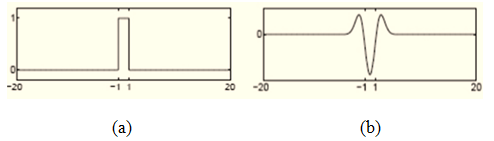
\includegraphics[width=0.60\textwidth]{fig/16.png}
    \vspace{-0.5em}   
    \begin{center}
    \caption{\textcolor{gray}{\footnotesize \textit{
    (a) En 3-D visualisering af en to-dimensional Laplacian of Guassian (b) ét en-dimensionalt signal (c) Laplacian of Gaussian operatoren anvendt på (b)}}}
    \label{fig:lapgauss}
     \end{center}
  \end{figure}
       \vspace{-2.5em}
\noindent
Som illustreret i \ref{fig:lindblob}(b) forekommer blobs, forekommer blobs i forskellige størrelser. Ligesom i virkeligheden, har objekter forskellige strukturer ift. hvor langt væk objektet er og kan derfor optræde anderledes, hvis de opfattes på forskellige skalaer. Blob detection skal derfor foregå på forskelligt skalaniveau i billedet, for at opnå skala-invariants. Skala-rummet i et 2-dimensionalt billede repræsenteres af flere billeder i forskellige skalaer af det originale billede. Billeder, der repræsentere forskellige skalaer, opnås ved at folde billedet med et 2-dimensionalt gaussisk filter som i \eqref{2dgaussian}. 
\begin{figure}[H]
    \centering
    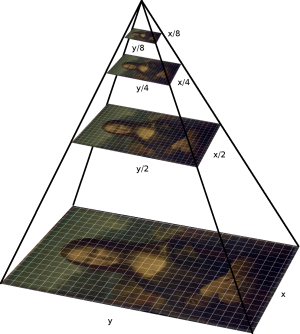
\includegraphics[width=0.35\textwidth]{fig/15.png}
    \vspace{-0.5em}   
    \begin{center}
    \caption{\textcolor{gray}{\footnotesize \textit{
En visualisering af et skala-rum formet som en pyramide af Leonardi Da Vinci's Mona Lisa. Hvert niveau angiver en skala repræsentation af det originale vindue, hvor toppen af pyramiden indeholder billeder af største skala og derfor med mindst information, og bunden af skalaen med det originale billede.
    }}}
    \label{fig:mona}
     \end{center}
  \end{figure}
       \vspace{-2.5em}
\noindent
Et gaussisk filter bruges da gradvis højere værdier af $\sigma$ fjerner strukturer, som vist i figur \ref{fig:sigma} og vigtigst af alt, at der ikke forekommer nye objekter ved transformationen fra finere til grovere skalaer \cite{lindenscale}. Billedet, der repræsentere flest detaljer, er den første skala, Idéen er derved at fjerne disse strukturer og, fremhæve andre objekter gradvist på en større skala der også kan detekteres. Detektionen af blobs sker altså på alle skalaer.
Et billede i skala rummet for billedet $f(x,y)$ kan derfor defineres som i \eqref{scalespace}
\begin{equation}
L(x,y,\sigma) = g(x,y,\sigma)\ast f(x,y)
\label{scalespace}
\end{equation}
hvor $g$ er det 2-dimensionelle gaussiske filter,$L(x,y,\sigma)$ repræsentere et et billede i skal-rummet, og skala-parametren $\sigma$, bestemmer skalaen, eller placeringen i skal pyramiden. $L(x,y,0) = f(x,y)$, da det er den "nederste" skala og den nederste del af skal pyramiden.
\section{Deskriptor}
\section{Deskriptor}
For at udvælge korresponderende punkter imellem billederne, skal interessepunkterne beskrives af en deskriptor $Des$. Deskriptoren er en funktion, der tager et billede og et punkt som input og returnerer en feature. Deskriptoren beskriver et interessepunkt ud fra information i og omkring punktet, og tilknytter punktet en feature $f$, i form af en n-dimensional vektor:
\begin{equation}
Des(I,p_i)=f_i
\end{equation}
\begin{equation}
Des(I',p_j')=f_j'
\end{equation}
For to korresponderende punkter $i$ og $j$ ønskes det at $f_i \approx f'_j$, så punkterne kan identificeres som værende korresponderende punkter, men også for to \textit{ikke} korresponderende punkter $k$ og $l$ at $f_k \not\approx f'_l$.
\section{Matching}
